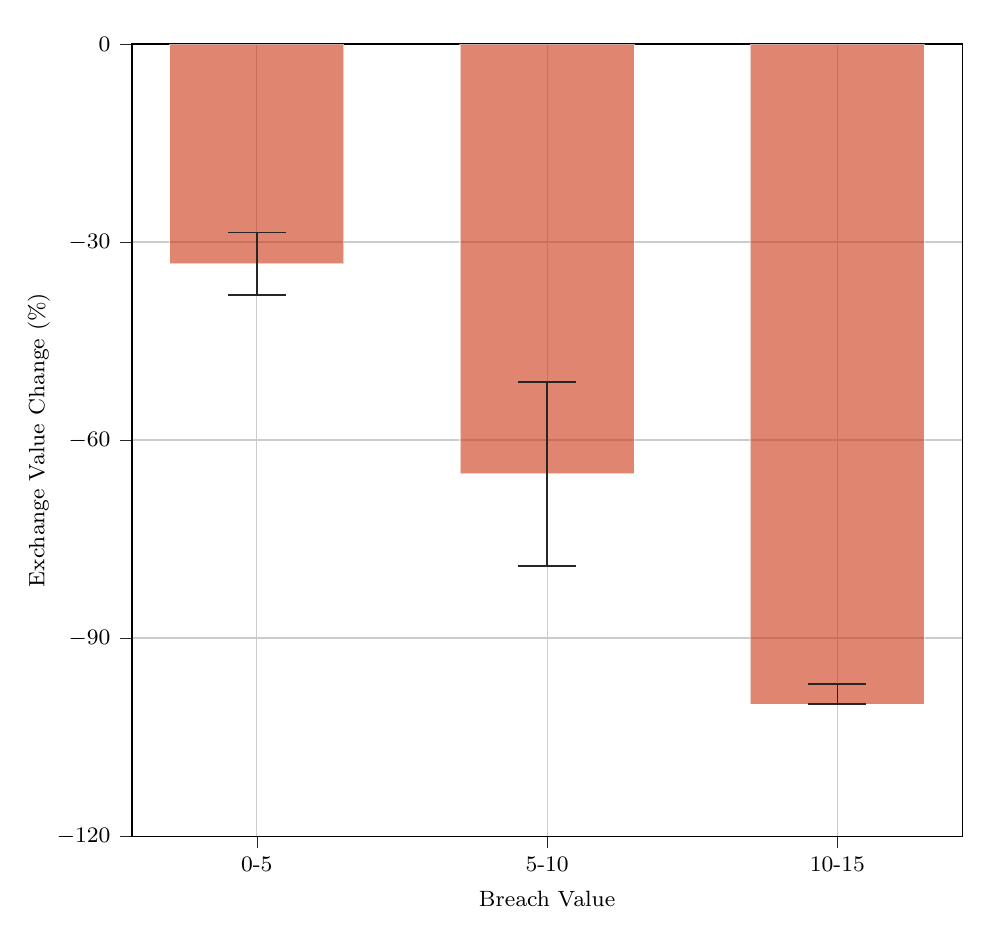
\begin{tikzpicture}
    \definecolor{darkslategrey38}{RGB}{38,38,38}
    \definecolor{darkslategrey66}{RGB}{66,66,66}
    \definecolor{lightgrey204}{RGB}{204,204,204}
    \definecolor{firebrick2045117}{RGB}{204,51,17}
    
    \begin{axis}[
        width=1\textwidth,    % 设置宽度
        height=0.96\textwidth,    % 16:9比例
        axis line style={black},
        tick align=outside,      % 刻度线向外
        anchor=north,
        at={(0,1)}, 
        axis lines=box,          % 显示完整边框
        tick pos=left,           % y轴刻度线只在左侧
        xtick pos=bottom,        % x轴刻度线只在底部
        clip=true,               % 裁剪超出内容
        unbounded coords=jump,
        x grid style={lightgrey204},
        xlabel=Breach Value,
        xlabel style={font=\footnotesize},
        xmajorticks=true,
        xmin=-0.43, xmax=2.43,
        xtick style={color=darkslategrey38},
        xtick={0,1,2},
        xticklabels={0-5,5-10,10-15},
        xticklabel style={font=\footnotesize,rotate=0},
        y grid style={lightgrey204},
        ylabel=Exchange Value Change (\%),
        ylabel style={font=\footnotesize,
            inner sep=0pt,    % 减少标签和轴的距离
            yshift=-1pt       % 微调标签位置
        },
        ymajorgrids,
        ymin=-120, ymax=0,
        ytick={-120,-90,-60,-30,0},
        yticklabel style={font=\footnotesize},
        ytick style={color=darkslategrey38},
        grid=major,
        grid style={lightgrey204},
        every outer x axis line/.append style={black},
        every outer y axis line/.append style={black}
    ]
    
    % 绘制柱状图
    \draw[draw=white,fill=firebrick2045117,opacity=0.6] 
        (axis cs:-0.3,0) rectangle (axis cs:0.3,-33.3017084294457);
    \draw[draw=white,fill=firebrick2045117,opacity=0.6] 
        (axis cs:0.7,0) rectangle (axis cs:1.3,-65.1388888888889);
    \draw[draw=white,fill=firebrick2045117,opacity=0.6] 
        (axis cs:1.7,0) rectangle (axis cs:2.3,-100);
    
    % 误差线
    % \path [draw=darkslategrey38, semithick]
    %     (axis cs:0,-38.0549349367552) -- (axis cs:0,-28.5484819221361);
    % \path [draw=darkslategrey38, semithick]
    %     (axis cs:1,-79.1065317716095) -- (axis cs:1,-51.1712460061683);
    % \path [draw=darkslategrey38, semithick]
    %     (axis cs:2,-97) -- (axis cs:2,-100);
    \draw[darkslategrey38, semithick] (axis cs:-0.1,-38.0549349367552) -- (axis cs:0.1,-38.0549349367552);
    \draw[darkslategrey38, semithick] (axis cs:0,-38.0549349367552) -- (axis cs:0,-28.5484819221361);
    \draw[darkslategrey38, semithick] (axis cs:-0.1,-28.5484819221361) -- (axis cs:0.1,-28.5484819221361);
    
    \draw[darkslategrey38, semithick] (axis cs:0.9,-79.1065317716095) -- (axis cs:1.1,-79.1065317716095);
    \draw[darkslategrey38, semithick] (axis cs:1,-79.1065317716095) -- (axis cs:1,-51.1712460061683);
    \draw[darkslategrey38, semithick] (axis cs:0.9,-51.1712460061683) -- (axis cs:1.1,-51.1712460061683);
    
    \draw[darkslategrey38, semithick] (axis cs:1.9,-97) -- (axis cs:2.1,-97);
    \draw[darkslategrey38, semithick] (axis cs:2,-97) -- (axis cs:2,-100);
    \draw[darkslategrey38, semithick] (axis cs:1.9,-100) -- (axis cs:2.1,-100);
    
    % 百分比标签
    % \node[above,font=\footnotesize\bfseries,text=firebrick2045117] 
    %     at (axis cs:0,-50.3017084294457) {-33.3\%};
    % \node[above,font=\footnotesize\bfseries,text=firebrick2045117] 
    %     at (axis cs:1,-90.1388888888889) {-65.1\%};
    % \node[above,font=\footnotesize\bfseries,text=firebrick2045117] 
    %     at (axis cs:2,-115) {-100.0\%};
        
\end{axis}
\end{tikzpicture}